\chapter{Выполнение работы:}
\section{Построение диаграммы классов}
\begin{figure}[ht] 
	\center
	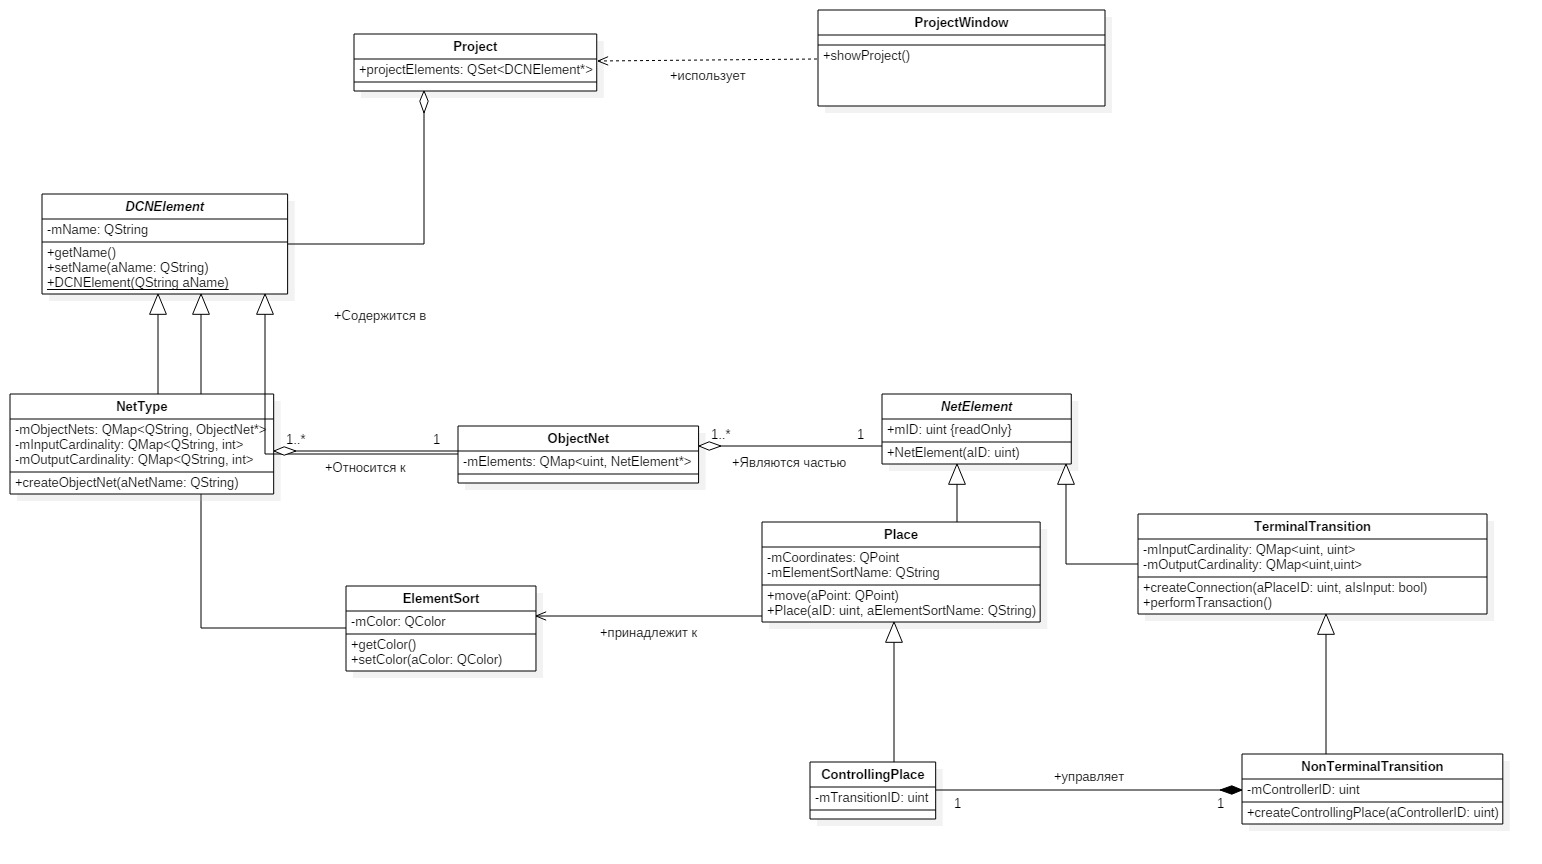
\includegraphics [width=\textwidth] {class}
	\caption{Диаграмма классов} 
\end{figure}
\FloatBarrier
\clearpage
\section{Построение диаграммы последовательности}

\begin{figure}[ht!] 
	\center
	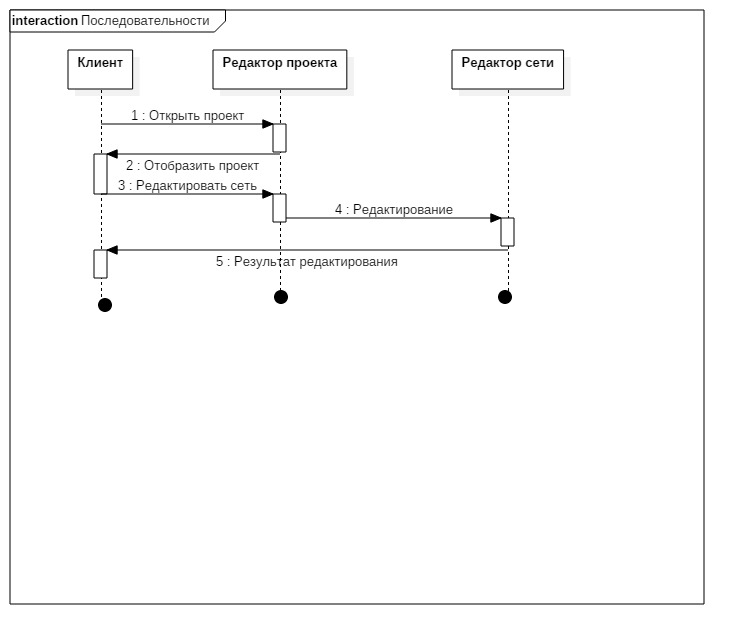
\includegraphics [width=\textwidth] {posled}
	\caption{Диаграмма последовательности} 
\end{figure}
\FloatBarrier
\clearpage
\section{Построение диаграммы кооперации}
\begin{figure}[ht] 
	\center
	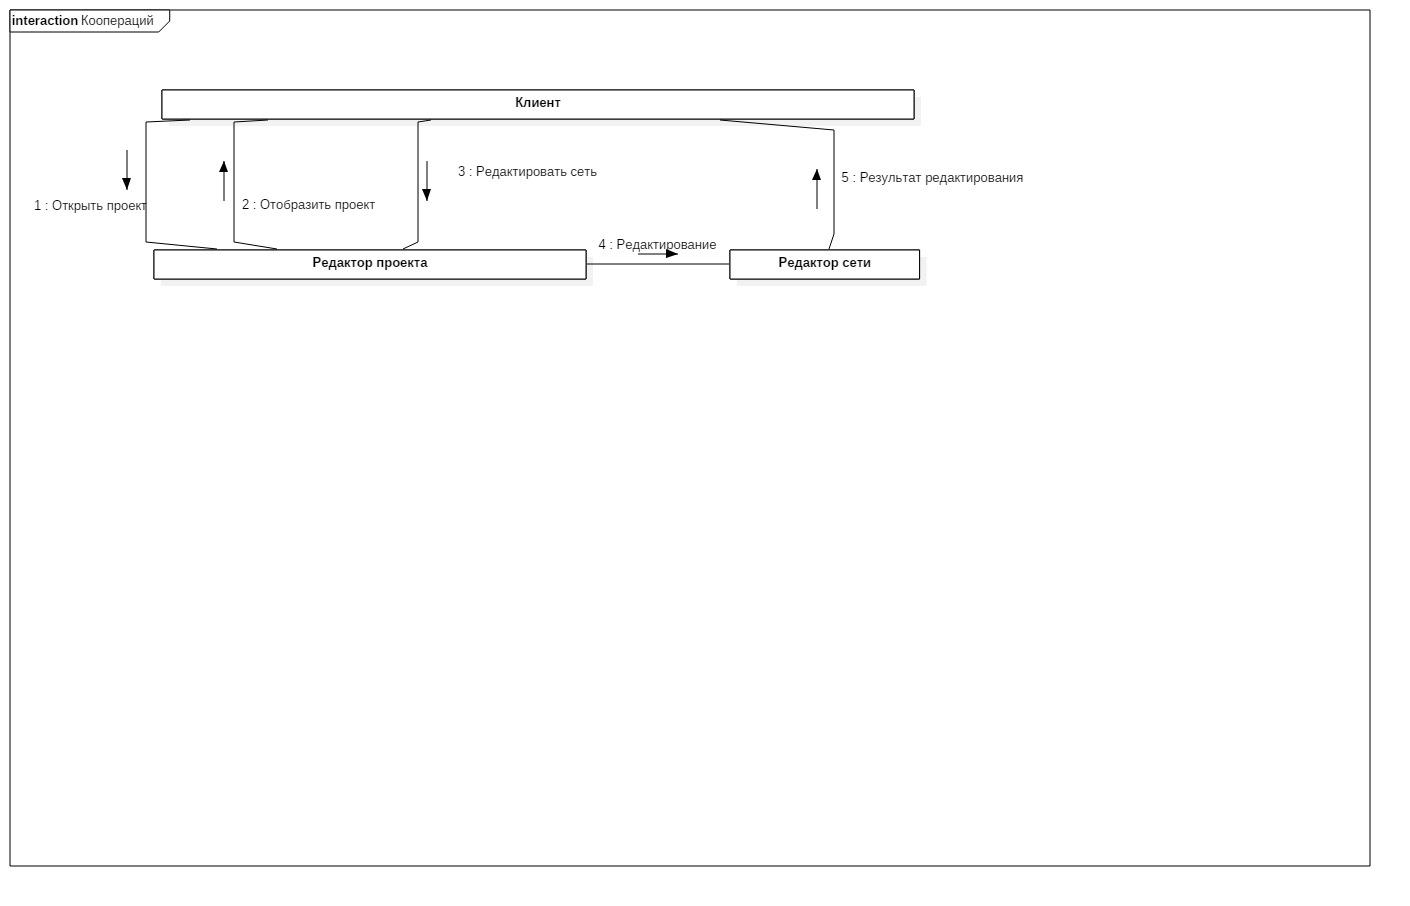
\includegraphics [width=\textwidth] {coop}
	\caption{Диаграмма кооперации} 
\end{figure}
\FloatBarrier
\clearpage
\section{Построение диаграммы деятельности}
\begin{figure}[ht] 
	\center
	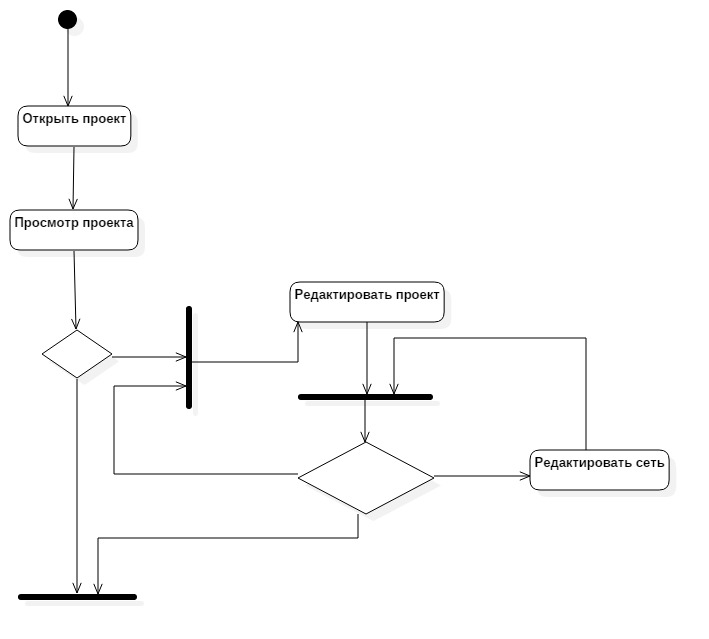
\includegraphics [width=\textwidth] {activity}
	\caption{Диаграмма деятельности} 
	
\end{figure}
\FloatBarrier
\clearpage
\section{Построение диаграммы состояний}
\begin{figure}[ht] 
	\center
	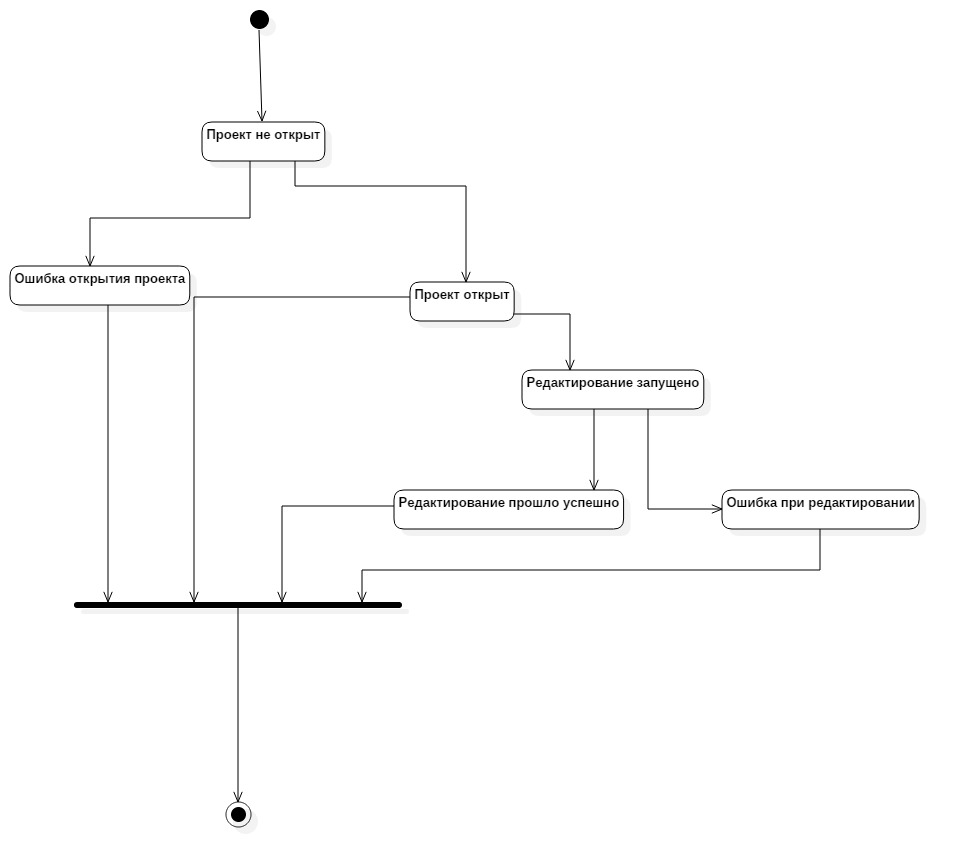
\includegraphics [width=\textwidth] {state}
	\caption{Диаграмма состояний} 
\end{figure}
